\documentclass{article}
\usepackage[utf8]{inputenc}

\usepackage{amsmath}
\usepackage{amsfonts}

\usepackage{hyperref}
\hypersetup{
    colorlinks=true,
    linkcolor=blue,
    filecolor=magenta,      
    urlcolor=cyan,
}

\usepackage{graphicx}
\graphicspath{{/home/karthik/Work/MS/courses/PR/assignment-4/}}
\setlength{\parindent}{0pt}

\title{Assignment-4 : Pattern Recognition}
\author{Arjun Manoharan (CS17S004) and Karthik Thiagarajan (CS16S027)}

\begin{document}

\maketitle

\tableofcontents

\newpage
\section{Isolated Digits}
\subsection{HMM}
\textbf{Data} : Classes given to us are ``1", ``5" and ``z".\\
\textbf{Algorithm} : The data is divided into train (70\%) and test (30\%). The data is quantized using K-means with the number of symbols being equal to the number of means. A left-right HMM is trained on each class. Given a test datapoint, the likelihood of all three HMM-models on this datapoint are obtained. The predicted class is the one having the maximum likelihood.\\
\textbf{Experiments} : The number of states and the number of symbols are the free variables. Each state-symbol combination corresponds to one experiment. The ROC-DET curves are plotted for all these models.

\begin{figure}[h!]
\centering
\title{Performance as a function of symbols}
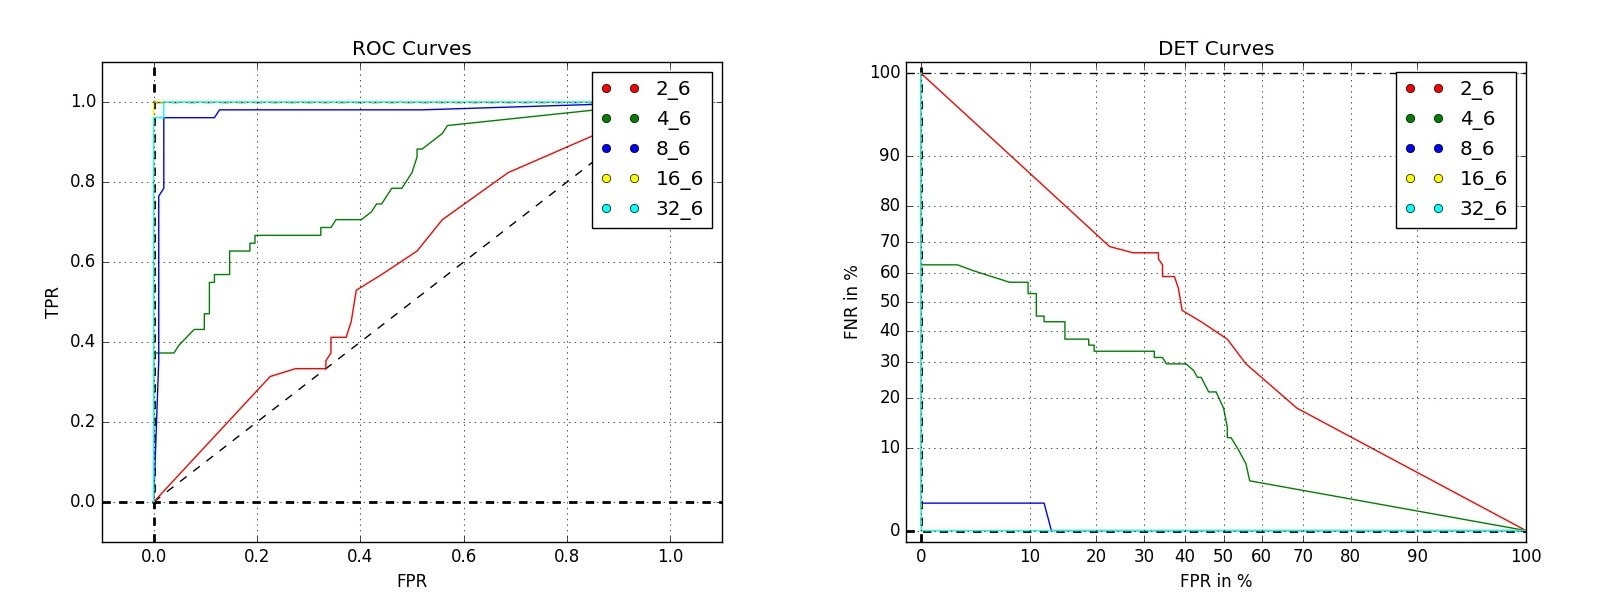
\includegraphics[width=\textwidth]{isolated_digits/plots/hmm/roc_det_symbols.jpg}
\caption{HMM is labelled as $<\text{symbols}>\_<\text{states}>$}
\end{figure}

\begin{figure}[h!]
\centering
\title{Performance as a function of states}
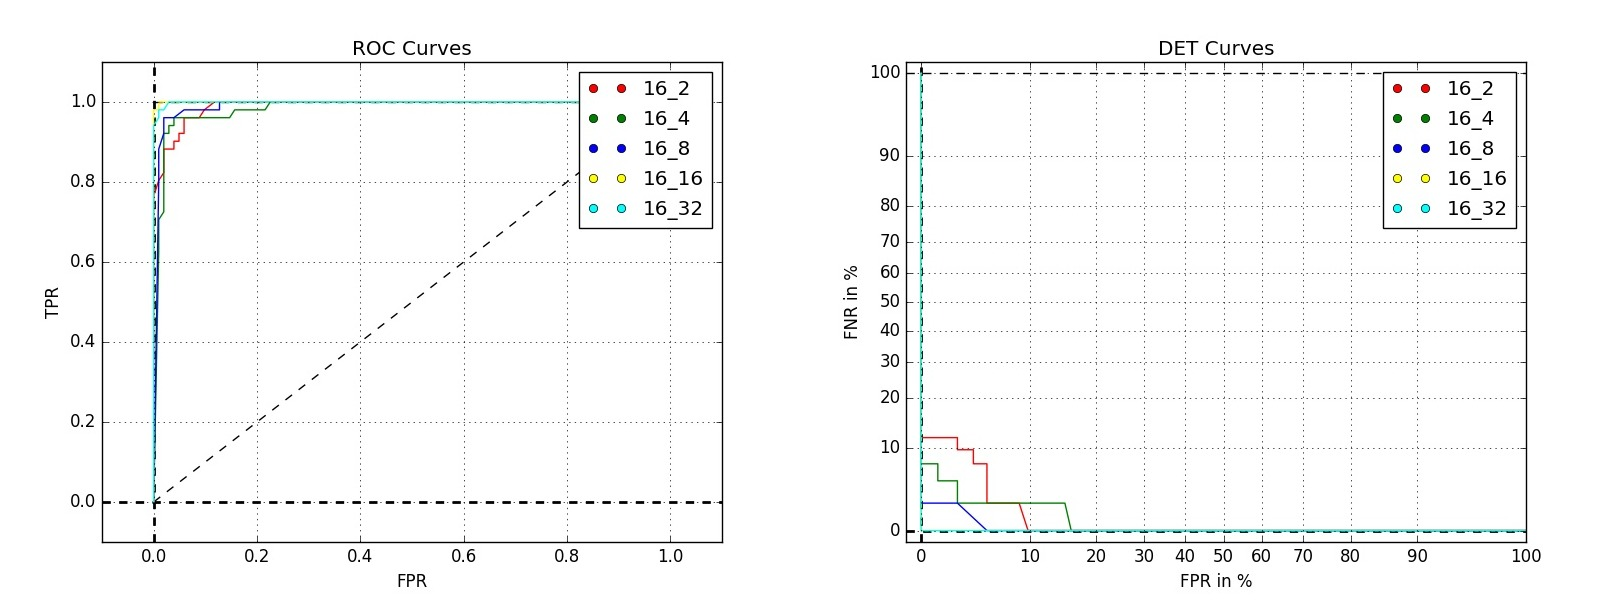
\includegraphics[width=\textwidth]{isolated_digits/plots/hmm/roc_det_states.jpg}
\caption{HMM is labelled as $<\text{symbols}>\_<\text{states}>$}
\end{figure}

\begin{figure}[h!]
\centering
\title{The best model}
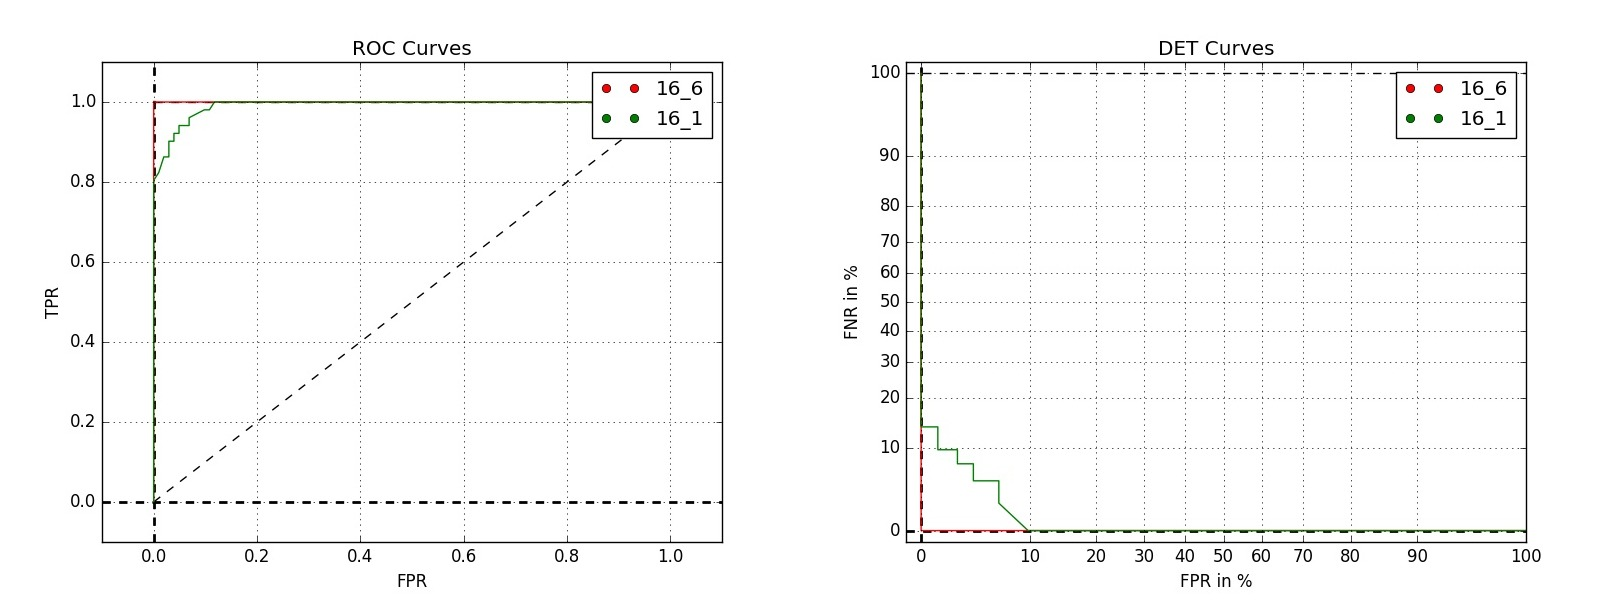
\includegraphics[width=\textwidth]{isolated_digits/plots/hmm/roc_det_final.jpg}
\caption{HMM is labelled as $<\text{symbols}>\_<\text{states}>$}
\end{figure}

\newpage
\textbf{Observations} : The design of the codebook has a much greater impact on the performance than that of the states. $16$ is observed to be the optimal codebook size. Even a single state HMM, 16-symbols HMM performs better than HMMs with a smaller codebook. 

\subsection{DTW}

\begin{figure}[h!]
\centering
\title{DTW-kNN classifier}
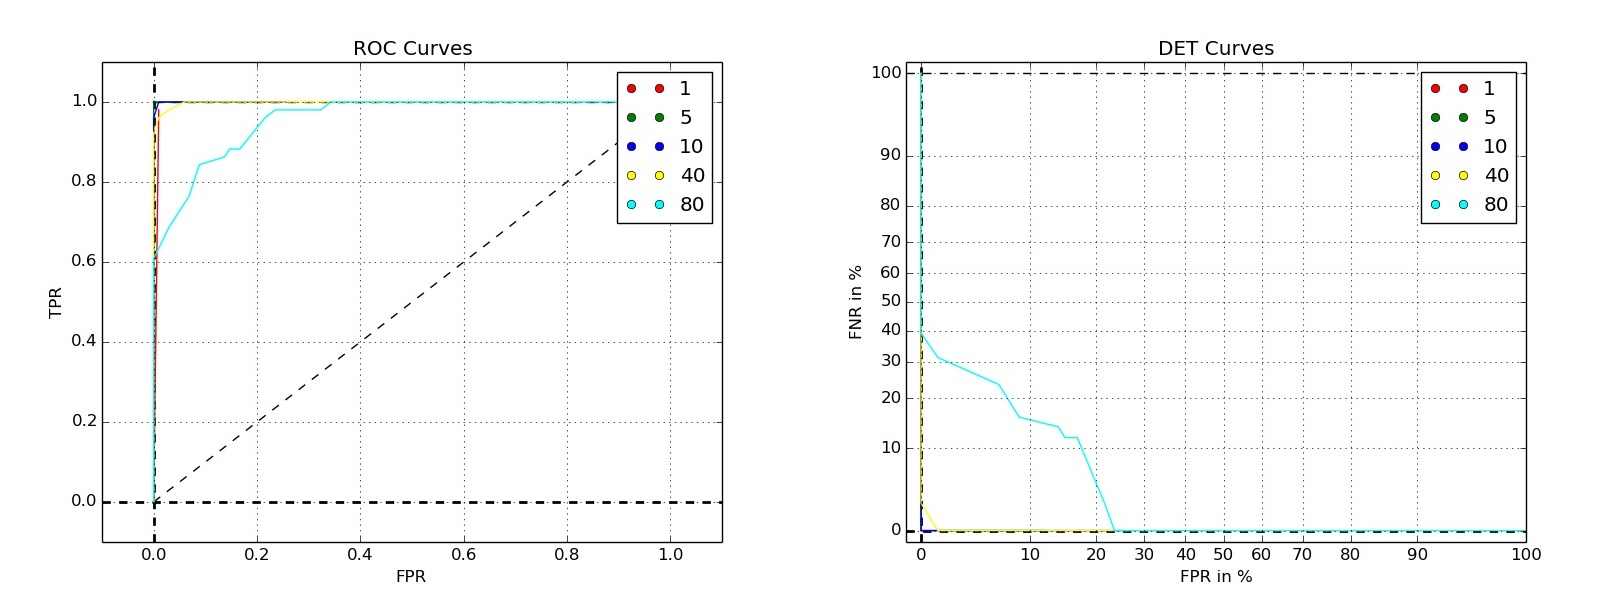
\includegraphics[width=\textwidth]{isolated_digits/plots/dtw/roc_det.jpg}
\caption{Each model is labelled by the number of nearest neighbours chosen.}
\end{figure}

\textbf{Observations} : Near perfect classification is obtained using just a single neighbour. This suggests that DTW is a very good distance measure for time series data.

\subsection{HMMs versus DTW}
\begin{itemize}
	\item No training or hyperparameter tuning required in DTW.
	\item Unlike HMMs, DTW is memory and compute intensive during test time.
	
\end{itemize}

\section{Connected Digits}

\begin{table}[h!]
\centering
\begin{tabular}{ |p{2.5cm}|p{2.5cm}|p{2.5cm}|  }
\hline
\multicolumn{3}{|c|}{Results on test-1} \\
\hline
Ground truth & Known model length & Unknown model length \\
\hline
11z & 11z & 11z\\
15 & 15 & 1555\\
15z & 1zz & 1zz\\
1z51 & 1z51 & 1z51z\\
1z & 1z & 1z5z1\\
1zz & 1zz & 1zz\\
1zzz1 & 1zzz1 & 1zzz1\\
51 & 51 & 511z1\\
51z & 51z & 51z1z\\
51zz5 & 51zz1 & 51zz1\\
55 & 55 & 55\\
z1 & z1 & z1zzz\\
z1z & zzz & zzz\\
z51z & z1z5 & z1z5\\
z5 & z5 & z51\\
z5z & z5z & z5z1\\
z5zzz & z5zzz & z5zzz\\
zz & zz & zz\\
\hline
\end{tabular}
\end{table}

\begin{table}[h!]
\centering
\begin{tabular}{ |p{2.5cm}|p{2.5cm}|p{2.5cm}|  }
\hline
\multicolumn{3}{|c|}{Results on test-2} \\
\hline
Ground truth & Fixed model length = 3 & Unknown model length \\
\hline
154.txt & 111 & 11\\
155.txt & 155 & 155z1\\
156.txt & 151 & 15151\\
157.txt & 1zz & 1zz15\\
158.txt & z51 & z51z1\\
159.txt & 551 & 55111\\
160.txt & 1zz & 1zz\\
161.txt & z1z & z1zzz\\
162.txt & zz5 & zz5z1\\
163.txt & zz5 & zz5z1\\
164.txt & zzz & zz\\
165.txt & zzz & zzz5z\\
166.txt & zzz & zzz\\
\hline
\end{tabular}
\end{table}

\newpage
16-symbol, 10-state HMM models trained on each class are used for this task. The HMMs are then concatenated to form different continuous models. During concatenation the final state's self-transition probability is set to 0.5, and its next state transition probability is also set to 0.5. Sequence lengths upto 5 are considered. So there are a total of $ 3^1 + 3^2 + 3^3 + 3^4 + 3^5 = 363$ HMM models against which each datapoint is tested.

\section{Handwriting}
\begin{figure}[h!]
\centering
\title{The characters}
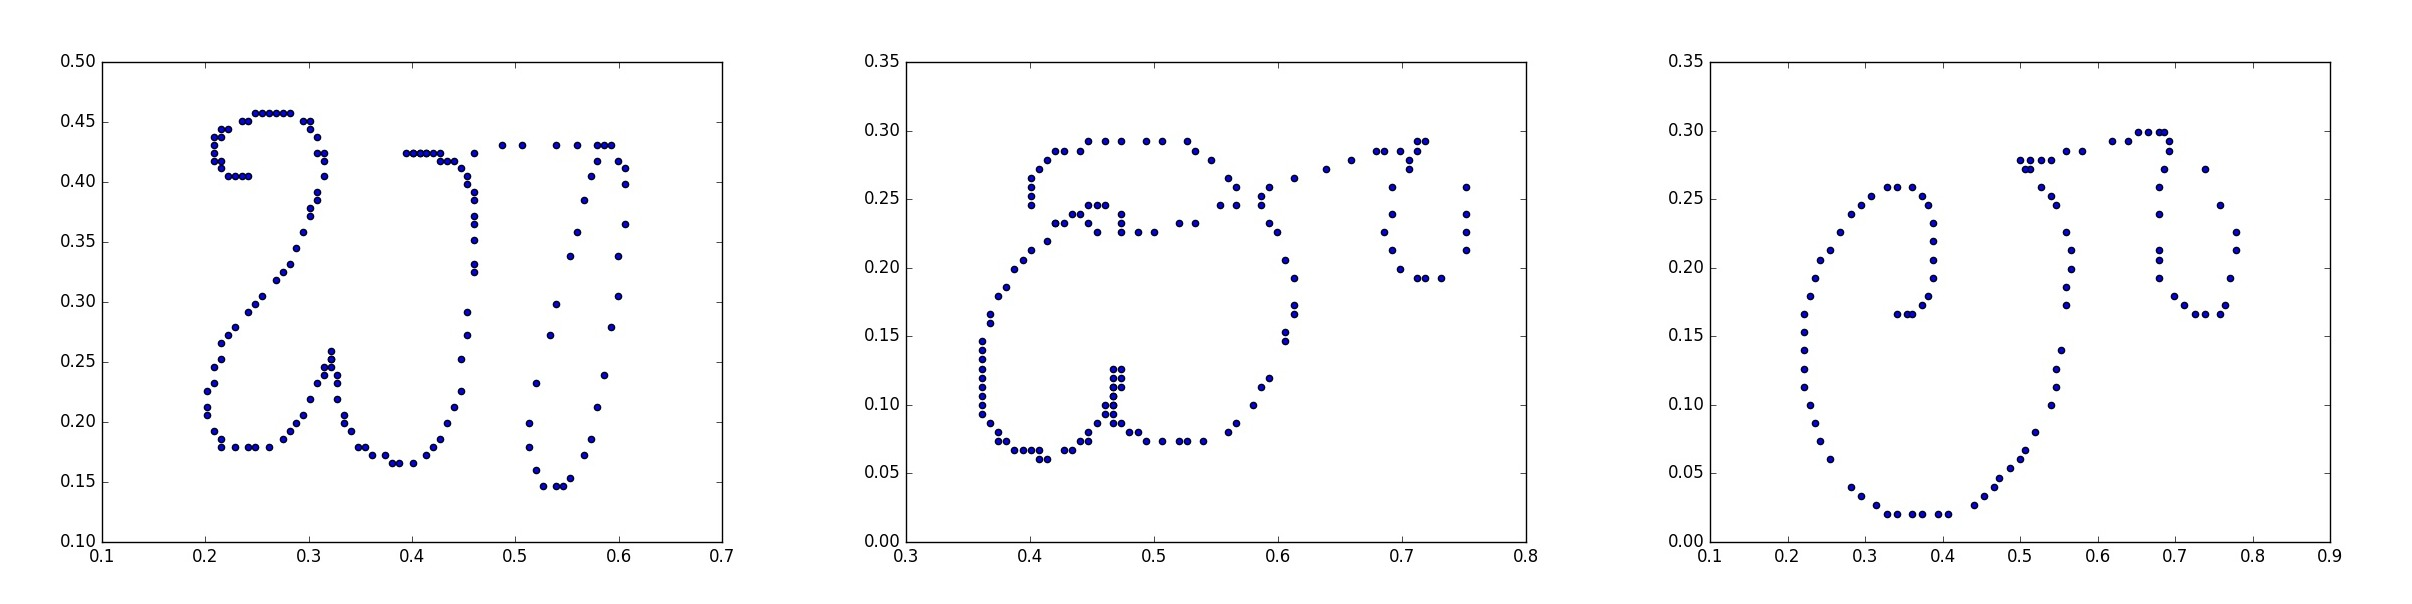
\includegraphics[width=\textwidth]{handwriting/plots/viz/train/bAdAlA.jpg}
\caption{bA, dA, lA}
\end{figure}
\subsection{HMM}
\subsubsection{Isolated}
\textbf{Isolated} : Four types of features are used : coordinates, first derivatives, second derivatives, curvature. Different combination of these features are used to prepare different datasets.

\begin{figure}[h!]
\centering
\title{The effect of curvature}
\includegraphics[width=\textwidth]{handwriting/plots/hmm/roc_det_x,y,kt.jpg}
\caption{HMM is labelled as $<\text{features}>\_<\text{symbols}>\_<\text{states}>$}
\end{figure}

\begin{figure}[h!]
\centering
\title{The effect of features on performance}
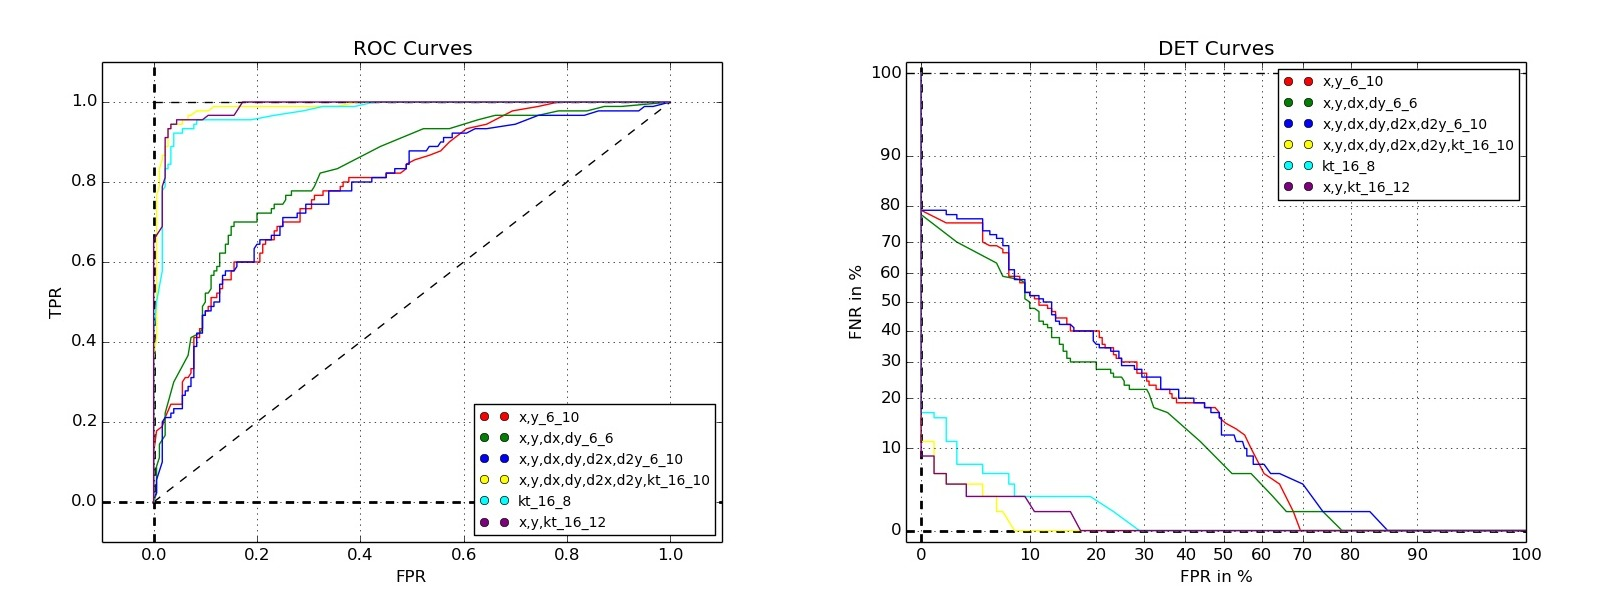
\includegraphics[width=\textwidth]{handwriting/plots/hmm/roc_det_compare.jpg}
\caption{HMM is labelled as $<\text{features}>\_<\text{symbols}>\_<\text{states}>$}
\end{figure}

\begin{table}[h!]
\centering
\begin{tabular}{ |p{1.5cm}|p{1.5cm}|p{1.5cm}|p{1.5cm}|  }
\hline
\multicolumn{4}{|c|}{Confusion Matrix on Test Data} \\
\hline
 & bA & dA & lA \\
\hline
bA & 29 & 1 & 0\\
dA & 0 & 30 & 0\\
lA & 0 & 5 & 25\\
\hline
\end{tabular}
\end{table}

\newpage
\textbf{Observations} : The curvature is the most important feature. The first and second derivatives capture the speed and acceleration of the stroke. Though the dataset has been generated in an online fashion by sampling points as they are written, the prediction happens offline, after the entire stroke has been recorded. Hence the speed and acceleration do not have any impact on the classification. In fact the second derivatives make the performance worse.\\
There is a confusion between the characters ``dA" and ``lA". Since the curvature is the main feature, we need to study the variation in curvature across a stroke for each of these characters. Though ``bA" and ``dA" have very similar curvatures for the second half of the stroke, the first halves have inverse curvature. This is a discriminating aspect.
\subsubsection{Continuous}
\begin{figure}[h!]
\centering
\title{1, 2 and 3}
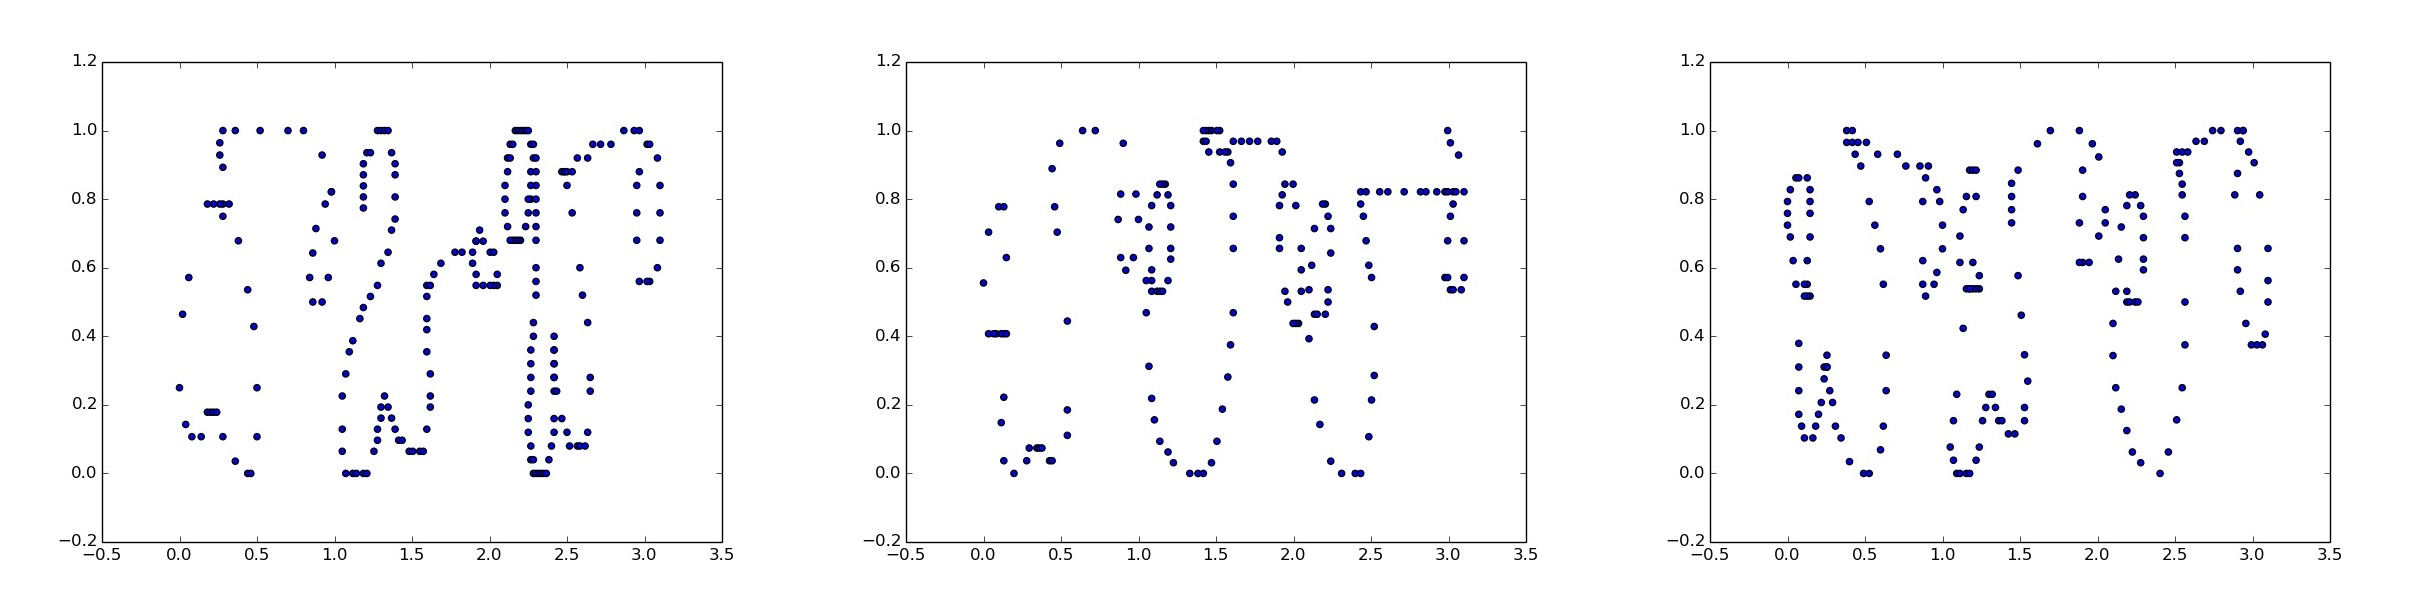
\includegraphics[width=\textwidth]{handwriting/plots/viz/123.jpg}
\end{figure}
\begin{table}[h!]
\centering
\begin{tabular}{ |p{2.5cm}|p{2.5cm}|p{3.5cm}|  }
\hline
\multicolumn{3}{|c|}{Results for 1, 2 and 3} \\
\hline
Ground truth & Fixed model length = 3 & Unknown model length \\
\hline
dA--bA--bA (1) & bA--dA--dA, bA--dA--bA, bA--dA--lA  & bA--dA--bA\\
bA--lA--lA (2) & \textbf{bA--lA--lA}, bA--lA--dA, bA--lA--bA & bA--lA--lA--bA--dA\\
bA--bA--lA (3) & dA--bA--bA & dA--bA--bA--dA\\
\hline
\end{tabular}
\end{table}


\subsection{DTW}
\begin{figure}[h!]
\centering
\title{DTW-kNN classifier}
\includegraphics[width=\textwidth]{handwriting/plots/dtw/roc_det_x,y,kt.jpg}
\caption{Each model is labelled by the number of nearest neighbours chosen}
\end{figure}

\begin{table}[h!]
\centering
\begin{tabular}{ |p{1.5cm}|p{1.5cm}|p{1.5cm}|p{1.5cm}|  }
\hline
\multicolumn{4}{|c|}{Confusion Matrix on Test Data} \\
\hline
 & bA & dA & lA \\
\hline
bA & 28 & 2 & 0\\
dA & 0 & 22 & 8\\
lA & 1 & 0 & 29\\
\hline
\end{tabular}
\end{table}


\end{document}